To produce predictions for the DCOs that are detectable with LISA, we synthesise a population of DCOs using the population synthesis methods described in Section~\ref{sec:COMPAS_explained}. In order to obtain value for the uncertainty on the expected detection rates, we place this sample of DCOS in many different Monte Carlo sampled instances of the Milky Way, the model for which is described in Section~\ref{sec:galaxy_synthesis}. We evolve the orbit of each DCO in a Milky Way instance up to the LISA mission and calculate the detection rate for that instance using the methods presented in Section~\ref{sec:gw_detection}.

\subsection{Binary population synthesis}\label{sec:COMPAS_explained}

We use a population of binaries recently presented in \citet{Broekgaarden+2021} and Broekgaarden et al. (in prep). This population is synthesised using the rapid population synthesis code \href{https://compas.science}{COMPAS}\footnote{\url{https://compas.science}} \citep{Stevenson+2017, Vigna-Gomez+2018, Stevenson+2019}. COMPAS follows the approach of the pioneering population synthesis code BSE \citep{Hurley+2000,Hurley+2002} and uses fitting formula and rapid algorithms to efficiently predict the final fate of millions of binary systems. The code is open source and documented in the papers listed above and the on-line documentation. An extensive method paper is forthcoming (Team COMPAS: J. Riley et al. (in prep)) We summarize the main assumptions and settings relevant for this work in the following sections.

\subsubsection{Initial conditions}

One million binaries are simulated for 50 metallicity bins equally spaced in log space between $Z \in [0.0001, 0.022]$, where $Z$ is the mass fraction of heavy elements. These bins span the allowed metallicities range for the original fitting formulae on which COMPAS is based \citep{Hurley+2000}. This is repeated for 14 physics variations (see Section \ref{sec:variation_assumptions}) and so in total 750 million binaries were simulated.

Each binary is sampled from initial distributions for the primary and secondary masses as well as the separation. The primary mass, that is the mass of the initially more massive star, is restricted to $m_1 \in [5, 150] \unit{M_{\odot}}$, which spans the range of interest for NS and BH formation in binary systems, and drawn from the \citet{Kroupa+2001} Initial Mass Function (IMF), $p(m_1) \propto m_1^{-2.3}$. The secondary mass is drawn using the mass ratio of the binary, which we assume to be uniform on $[0, 1]$, therefore $p(q) = 1$ \citep[consistent e.g. with][]{Sana+2012}. We additionally restrict $m_2 \ge 0.1 \unit{M_{\odot}}$, since this is approximately the minimal mass for a main sequence star. We assume that the initial separation follows a flat in the log distribution with $p(a_i) \propto 1 / a_i$ and $a_i \in [0.01, 1000] \unit{AU}$ \citep{Opik+1924, Abt+1983}. We assume that all binaries are circular at birth to reduce the dimensions of initial parameters. Since we focus on post-interaction binaries which will have circularised during mass transfer this is a reasonable assumption and is likely not critical for predicting detection rates \citep{Hurley+2002, deMink+2015}. In addition, we apply the adaptive importance sampling algorithm STROOPWAFEL \citep{Broekgaarden+2019} to improve the yield of our sample. This algorithm increases the prevalence of target DCOs (BHBHs, BHNSs and NSNSs in this case) in the sample and assigns each a weight, $w$, which represents the probability of drawing it without STROOPWAFEL in effect.

For each metallicity $Z$, we thus have a sample of binaries, each with a set of parameters
\begin{equation}
    \mathbf{b}_{{Z, i}} = \{m_1, m_2, a_{\rm DCO}, e_{\rm DCO}, t_{\rm evolve}, t_{\rm inspiral}, w\},
\end{equation}
for $i = 1, 2, \dots, N_{\rm binary}$, where $m_1$ and $m_2$ are the primary and secondary masses, $a_{\rm DCO}$ and $e_{\rm DCO}$ are the semi-major axis and eccentricity at the moment of double compact object (DCO) formation, $t_{\rm evolve}$ is the time between the binary's zero-age main sequence and DCO formation, $t_{\rm inspiral}$ is the time between DCO formation (that is immediately after the second supernova in the system) and gravitational wave merger, $w$ is the adaptive importance sampling weight assigned by STROOPWAFEL. We sample from these sets of parameters when creating synthetic galaxies.

\subsubsection{Physical assumptions in fiducial model}\label{sec:fiducial_physics}
In this section we briefly summarise the main physical assumptions in our fiducial model. For more details see \citet{Broekgaarden+2021}.

\textit{Stellar Evolution:} To follow the evolution of massive stars, COMPAS relies on fitting formula by \citet{Hurley+2000} to detailed single star models by \citet{Pols+1998}. COMPAS implements stellar wind mass loss using the prescriptions from \citet{Belczynski+2010b} and models the evolution of stars that lose or gain mass closely following the algorithms originally described in \citet{Tout+1996} and \citet{Hurley+2002}. For more information about the implementation of the single star evolution in COMPAS see the corresponding section in the upcoming methods paper (Team COMPAS: J. Riley et al. (in prep)).

\textit{Mass Transfer:} In determining the stability of mass transfer we use the $\zeta$-prescription, which compares the radial response of the star with the response of the Roche lobe radius to the mass transfer \citep[e.g.][]{Hjellming+1987}. The mass transfer efficiency, $\beta = \Delta M_{\rm acc} / \Delta M_{\rm don}$, is defined as the fraction of the mass transferred by the donor that is actually accreted by the accretor. We limit the maximum accretion rate for stars to $\Delta M_{\rm acc} / \Delta t \le 10 M_{\rm acc} / \tau_{\rm KH}$, where $\tau_{\rm KH}$ is the Kelvin-Helmholtz timescale of the star \citep{Paczynski+1972, Hurley+2002}. The maximum accretion rate for double compact objects is limited to the Eddington accretion rate. If more mass than these rates is accreted then we assume that the excess is lost through isotropic re-emission in the vicinity of the accreting star, thus varying $\beta$ \citep[e.g.][]{Massevitch+1975, Soberman+1997}. We assume that all mass transfer phases from a stripped post-helium-burning-star (case BB) onto a neutron star or black hole are unstable \citep{Tauris+2015}.

\textit{Common Envelope:} A common envelope phase follows dynamically unstable mass transfer and we parameterise this using the $\alpha$-$\lambda$ prescription from \citet{Webbink+1984} and \citet{deKool+1990}. We assume $\alpha = 1$, such that all of the gravitational binding energy is available for the ejection of the envelope. For $\lambda$ we use the fitting formulae from \citet{Xu+2010, Xu+2010a}. We assume that any Hertzsprung gap donor stars that initiate a common envelope phase will not survive this phase due to a lack of a steep density gradient between the core and envelope \citep{Taam+2000, Ivanova+2004}. This follows the `pessimistic' common envelope scenario \citep[c.f.][]{Belczynski+2007}. We remove any binaries where the secondary immediately fills its Roche lobe upon the conclusion of the common envelope phase as we treat these as failed common envelope ejections.

\textit{Supernovae:} We draw the remnant masses and natal kick magnitudes from different distributions depending on the type of supernova that occurs. For stars undergoing a general core-collapse supernova, we use the \textit{delayed} supernova remnant mass prescription from \citet{Fryer+2012}. The \textit{delayed} prescription does not reproduce the neutron star black hole mass gap and we use this as our default as it has been shown to provide a better fit for observed populations of DCOs \citep[e.g.][]{Vigna-Gomez+2018}. We draw the natal kick magnitudes from a Maxwellian velocity distribution with a one-dimensional root-mean-square velocity dispersion of $\sigma_{\rm rms}^{\rm 1D} = 265 \unit{km}{s^{-1}}$ \citep{Lyne+1994, Hobbs+2005}.

We assume that stars with helium core masses between $1.6$--$2.25 \unit{M_{\odot}}$ \citep{Hurley+2002} experience electron-capture supernovae \citep{Nomoto+1984, Nomoto+1987, Ivanova+2008}. We set all remnant masses to $1.26 \unit{M_{\odot}}$ in this case as an approximation of the solution to Equation 8 of \citet{Timmes+1996}. For these supernovae, we set $\sigma_{\rm rms}^{\rm 1D} = 30 \unit{km}{s^{-1}}$ as in \citet{Pfahl+2002} and \citet{Podsiadlowski+2004}.

We assume that stars that undergo case BB mass transfer \citep{Dewi+2002} experience extreme stripping which leads to an ultra-stripped supernova \citep{Tauris+2013, Tauris+2015}. For these supernovae we calculate the remnant mass using the \citet{Fryer+2012} prescription and use $\sigma_{\rm rms}^{\rm 1D} = 30 \unit{km}{s^{-1}}$ (as with electron-capture supernovae).

Stars with final helium core masses between $60$-$135 \unit{M_{\odot}}$ are presumed to undergo a pair-instability, or pulsational pair-instability supernova \citep[e.g.][]{Woosley+2007, Farmer+2019}. We follow the prescription from \citet{Marchant+2019} as implemented in \citep{Stevenson+2019} for these supernovae.

We assume that kicks are isotropic in the frame of the collapsing star. We adopt a maximum neutron star mass of $2.5 \unit{M_{\odot}}$ \citep[e.g.][]{Kalogera+1996, Fryer+2015, Margalit+2017} for the fiducial model and change the \citet{Fryer+2012} prescription accordingly.

\subsubsection{Model variations} \label{sec:variation_assumptions}
In addition to our fiducial model for the formation of DCOs, we explore 14 other models in which we change various aspects of the mass transfer, common envelope and supernova physics assumptions in order to assess the effect of their uncertainties on the overall double compact object detection rates and distributions. Each of the models varies a single physics assumption (fiducial assumptions are outlined in Section~\ref{sec:fiducial_physics}) and these are outlined in Table~\ref{tab:physics_variations}.

Our fiducial model is labelled model \modFid{}. Models \modRangeMT{} focus on changes to the mass transfer physics assumptions. We explore the effect of fixing the mass transfer efficiency $\beta$ to a constant value, rather than allowing it to vary based on the maximum accretion rate. In models \modBetaLow{}, \modBetaMed{}, \modBetaHigh{}, in which we set the value of $\beta$ to $0.25$, $0.5$ and $0.75$ respectively. In model \modCaseBB{} we investigate the consequence of assuming that case BB mass transfer onto a neutron star or black hole is always stable rather than always unstable.

Models \modRangeCE{} focus on altering the common envelope physics. We change the common envelope efficiency parameter in models \modAlphaLow{} and \modAlphaHigh{} to $\alpha = 0.5$ and $2.0$ respectively. In model \modOpt, we relax our restriction that Hertzsprung gap donor stars cannot survive common envelope events, thereby following the `optimistic' common envelope scenario.

Finally, in models \modRangeSN{} we consider changes related to our assumptions about supernova physics. Model \modRapid{} uses the alternate \textit{rapid} remnant mass prescription from \citet{Fryer+2012} instead of the \textit{delayed} prescription. We change the maximum neutron star mass in models \modNSLow{} and \modNSHigh{} to $2$ and $3 \unit{M_{\odot}}$ respectively to account for the range of predicted maximum neutron star masses. Model \modNoPISN{} removes the implementation of pair-instability and pulsational pair-instability supernovae. In models \modSigLow{} and \modSigLower{} we decrease the root-mean-square velocity dispersion for core-collapse supernovae to explore the effect of lower kicks. Finally, model \modNoBH{} removes the natal kick for all black holes.

\begin{table}[htb]
    \centering
    \begin{tabular}{cl}
        \hline \hline
        Model & Physics Variation \\
        \hline \hline
        \modFid & Fiducial (see Section~\ref{sec:fiducial_physics}) \\
        \hline
        \modBetaLow & Fixed mass transfer efficiency of $\beta=0.25$ \\ 
        \modBetaMed & Fixed mass transfer efficiency of $\beta=0.5$  \\ 
        \modBetaHigh & Fixed mass transfer efficiency of $\beta=0.75$ \\ 
        \modCaseBB & Case BB mass transfer is always unstable \\
        \hline
        \modAlphaLow & CE efficiency parameter $\alpha = 0.5$ \\
        \modAlphaHigh & CE efficiency parameter $\alpha = 2$   \\
        \modOpt & HG donor stars initiating a CE survive CE \\
        \hline
        \modRapid & Fryer rapid SN remnant mass prescription \\
        \modNSLow & Maximum NS mass is fixed to $2\unit{M_{\rm odot}}$ \\
        \modNSHigh & Maximum NS mass is fixed to $3\unit{M_{\rm odot}}$ \\
        \modNoPISN & PISN and pulsational-PISN not implemented \\
        \modSigLow & $\sigma_{\rm{rms}}^{\rm{1D}}=100 \unit{km}{s^{-1}}$ for core-collapse supernova \\  
        \modSigLower & $\sigma_{\rm{rms}}^{\rm{1D}}=30  \unit{km}{s^{-1}}$ for core-collapse supernova \\ 
        \modNoBH & Black holes receive no natal kick \\
        \hline \hline
    \end{tabular}%
    \caption{A description of the 15 binary population synthesis models used in this study. \modFid{} is the fiducial model, \modRangeMT{} change mass transfer physics, \modRangeCE{} change common envelope physics and \modRangeSN{} change supernova physics \citep[c.f.][Table 2]{Broekgaarden+2021}.}
    \label{tab:physics_variations}
\end{table}

\subsection{Galaxy synthesis}\label{sec:galaxy_synthesis}

In order to estimate a detection rate of DCOs with statistical uncertainties, we create a series of random instances of the Milky Way, each populated with a subsample drawn (with replacement) from the synthesised binaries described in Section~\ref{sec:COMPAS_explained}.

Most previous studies that predict a detection rate for LISA place binaries in the Milky Way independently of their age or evolution. We improve upon this as the first study to use an empirically-informed analytical model of the Milky Way that takes into account the galaxy's enrichment history by applying the metallicity-radius-time relation from \citet{Frankel+2018}. The authors developed this relation in order to measure the global efficiency of radial migration in the Milky Way and calibrated it using a sample of red clump stars measured with APOGEE \citep{Majewski+2017}.
%and matched to stars in Gaia \citep{GaiaCollaboration+2016}.

In Section~\ref{sec:mw_model}, we outline our model for the Milky Way and in Section~\ref{sec:combining_pop_gal} we explain how we combine our population of synthesised DCOs with this Milky Way model.

\subsubsection{Milky Way model}\label{sec:mw_model}

\begin{figure*}[t]
    \centering
    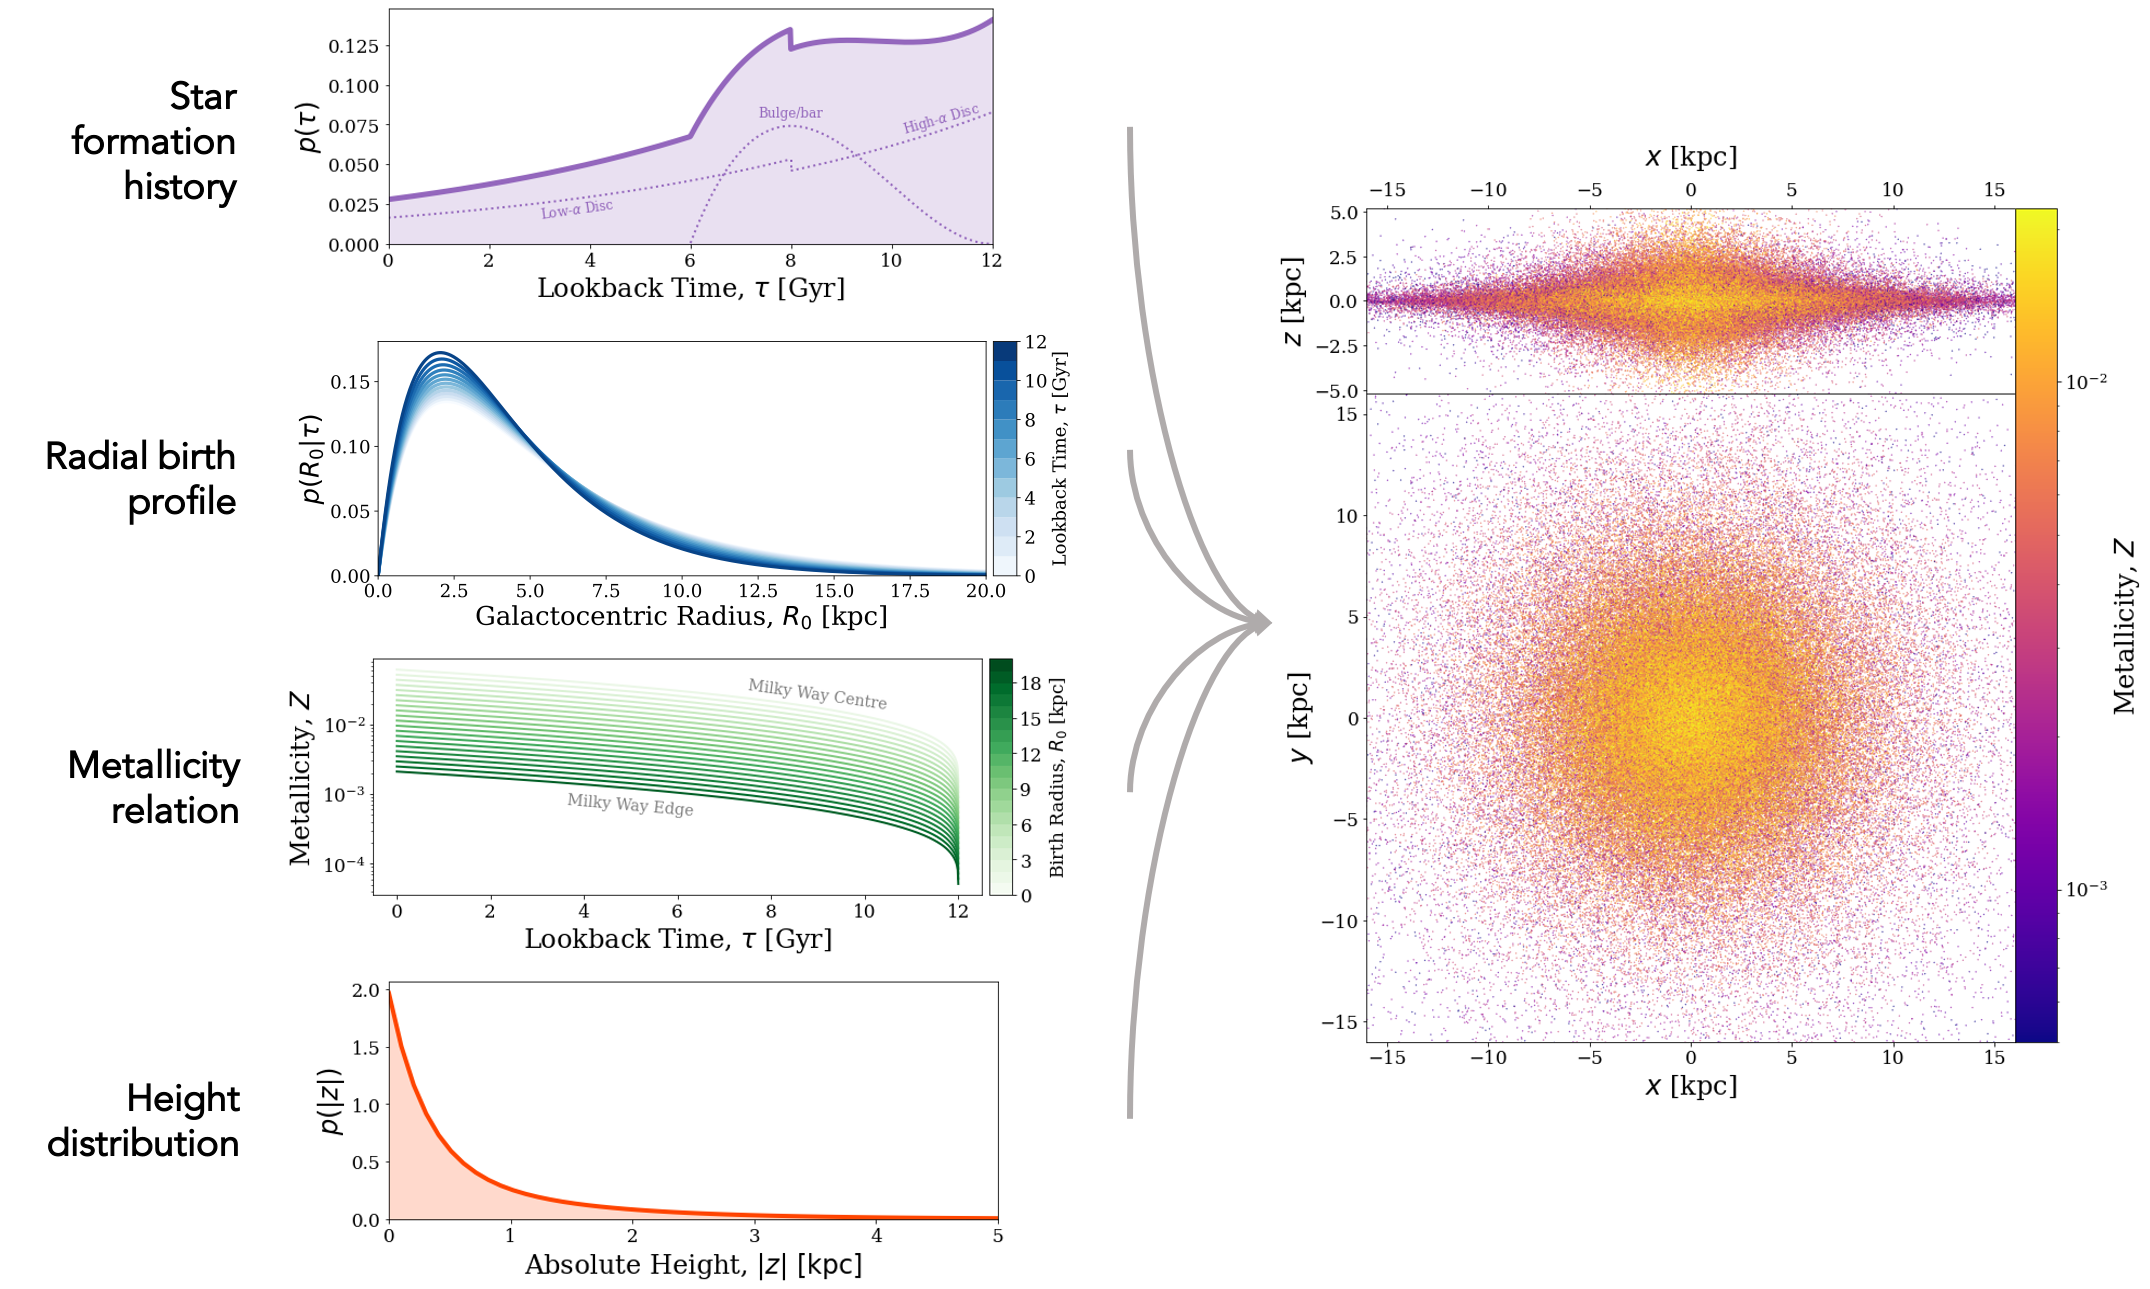
\includegraphics[width=\textwidth]{1_galaxy_diagram.png}
    \caption{A schematic illustrating how we create a mock Milky Way galaxy. The left panel illustrates the different model aspects: star formation history of 3 galactic components (individually shown in the dotted lines), spatial distribution at birth, age-metallicity-radius relation, and vertical distribution.
    On the right, we show an example instance of the Milky Way with $10^5$ binaries shown as points colour coded by metallicity. The top panel shows a side-on view and the bottom panel shows a face-on view.}
    \label{fig:galaxy_schematic}
\end{figure*}

Our model for the Milky Way accounts for the low-$\alpha$ disc, high-$\alpha$ disc and central bar/bulge. For each of these components, we use a separate star formation history, radial and vertical distribution, which we combine into a single model, weighting each component by its stellar mass. \citet{Licquia+2015} gives that the stellar mass of the bulge is $0.9 \times 10^{10} \unit{M_{\odot}}$ and the stellar mass of the disc is $5.2 \times 10^{10} \unit{M_\odot}$, which we split equally between the low- and high-$\alpha$ discs \citep[e.g.,][]{Snaith+2014}.

\textit{Star formation history:} 
We use an exponentially declining star formation history \citep{Frankel+2018} (a priori inspired by average the cosmic star formation history) for the combined low- and high-$\alpha$ disks, where the two disks transition at about 8 Gyr ago, and re-normalize the produced mass to be equal in each of the two components.
\begin{equation}\label{eq:thin_disc_tau}
    p(\tau) \propto \exp \qty(-\frac{(\tau_m - \tau)}{\tau_{\rm SFR}}),
\end{equation}
where $\tau$ is the lookback time (the amount of time elapsed between the binary's zero-age main sequence and today), $\tau_m = 12 \unit{Gyr}$ is the assumed age of the Milky Way and $\tau_{\rm SFR} = 6.8 \unit{Gyr}$ is the star formation timescale. 

The star formation history of the Milky Way bulge (which we assume here to be dominated by the central bar) has many uncertainties due to (1) sizeable age measurement uncertainties at large ages in observational studies, (2) complex selection processes affecting the observed age distributions, and (3) formation mechanisms still under debate. But the bulge was shown to contain stars with a range of 6-12 Gyr \citep[e.g.,][]{Bovy+2019}, where the younger tail of ages might come from the growth of the Galactic bar. To model the bulge age distribution more realistically than in previous studies (assuming an older bulge coming from a single starburst), we choose to adopt a star formation history using a $\beta(2,3)$ distribution, shifted and scaled such that stars are only formed in the range $[6, 12] \unit{Gyr}$

\textit{Radial distribution:} For each of the three components we employ the same single exponential distribution (but with different scale lengths)
\begin{equation}\label{eq:galaxy_R}
    p(R) = \exp(-\frac{R}{R_d}) \frac{R}{R_d^2},
\end{equation}
where $R$ is the Galactocentric radius and $R_d$ is the scale length of the component. For the low-$\alpha$ disc, we set $R_d = R_{\rm exp}(\tau)$, where $R_{\rm exp}(\tau)$ is the scale length presented in \citet[][Eq.~5]{Frankel+2018}
\begin{equation}
    R_{\rm exp}(\tau) = 4 \unit{kpc} \qty(1 - \alpha_{R_{\rm exp}} \qty(\frac{\tau}{8 \unit{Gyr}})),
\end{equation}
where $\alpha_{R_{\rm exp}} = 0.3$ is the inside-out growth parameter\footnote{In $R_{\rm exp}(\tau)$, we use 4 kpc instead of 3 kpc for the 0 Gyr exponential scale-length of the disc as NF finds that it provides a better fit to the original data}. This scale length accounts for the inside-out growth of the low-$\alpha$ disc and hence is age dependent. We assume $R_d = (1 / 0.43) \unit{kpc}$ for the high-$\alpha$ disc \citep[][Table~1]{Bovy+2016} and $R_d = 1.5 \unit{kpc}$ for the bar component \citep{Bovy+2019}.

\textit{Vertical distribution}: Similar to the radial distribution, we use the same single exponential distribution (but with different scale heights) for each component
\begin{equation}\label{eq:galaxy_z}
    p(\abs{z}) = \frac{1}{z_d} \exp\qty(-\frac{z}{z_d}),
\end{equation}
where $z$ is the height above the Galactic plane and $z_d$ is the scale height. We set $z_d = 0.3 \unit{kpc}$ for the low-$\alpha$ disc \citep{McMillan+2011} and $z_d = 0.95 \unit{kpc}$ for the high-$\alpha$ disc \citep{Bovy+2016}. 
\todo{Neige to Tom: for bar, I will think more for your bar scale-height, but the exact value should not change your results much since they will only slightly change the distance distribution of your sources, but not the rates nor the normalization.}
For the bulge, we set $z_d = 1.5 \unit{kpc}$ such that the probability of forming a star approaches zero at approximately the co-rotation radius of the Galactic bar/bulge \citep{Bovy+2019}. \todo{@Neige, did I justify the bulge/bar height correctly? A: The vertical distribution should not influence at which radius the bar should stop forming stars -- more later}

\textit{Metallicity-radius-time relation:} The relation is given by \citep[][Eq. 7]{Frankel+2018}
\begin{equation}\label{eq:galaxy_FeH}
    \begin{split}
        [{\rm Fe} / {\rm H}] (R, \tau) &= F_m + \nabla [{\rm Fe} / {\rm H}] R \\
        &- \qty(F_m + \nabla [{\rm Fe} / {\rm H}] R^{\rm now}_{[{\rm Fe} / {\rm H}] = 0} ) f(\tau),
    \end{split}
\end{equation}
where
\begin{equation}
    f(\tau) = \qty(1 - \frac{\tau}{\tau_m})^{\gamma_{[{\rm Fe} / {\rm H}]}},
\end{equation}
$F_m = -1 \unit{dex}$ is the metallicity of the gas at the center of the disc at $\tau = \tau_m$, $\nabla [{\rm Fe} / {\rm H}] = -0.075 \unit{kpc^{-1}}$ is the metallicity gradient, $R^{\rm now}_{[{\rm Fe} / {\rm H}] = 0} = 8.7 \unit{kpc}$ is the radius at which the present day metallicity is solar and $\gamma_{[{\rm Fe} / {\rm H}]} = 0.3$ set the time dependence of the chemical enrichment. We can convert this to the representation of metallicity that we use in this paper by applying \citep[e.g][]{Bertelli+1994}
\begin{equation}\label{eq:galaxy_FeH_to_Z}
    \log_{10} (Z) = 0.977 [{\rm Fe} / {\rm H}] + \log_{10}(Z_\odot).
\end{equation}

Although \citet{Frankel+2018} only fit this model for the low-$\alpha$ disc, we also use this metallicity-radius-time relation for the high-$\alpha$ disk and the bar, but focusing on the chemical tracks more representative to the inner disk and large ages. \citet{Sharma+2020} showed that using a simple continuous model for both the low- and high-$\alpha$ discs, the Milky Way abundance distributions could be well reproduced. Empirically, the chemical tracks in the [$\alpha$/Fe]-[Fe/H] plane of the stars in the bulge/bar follow the same track as those of the old stars in the Solar neighbourhood \citep[][Fig.~7,]{Bovy+2019}, which motivates our modelling choice to use the same metallicity-radius-time relation.

Fig.~\ref{fig:galaxy_schematic} shows the distributions and relations outlined in this section and also displays an example random galaxy drawn using this model.

\subsubsection{Combining population and galaxy synthesis}\label{sec:combining_pop_gal}

For each Milky Way instance, we randomly sample the following set of parameters
\begin{equation}
    \mathbf{g}_{{i}} = \{\tau, R, Z, z, \theta\}
\end{equation}
for $i = 1, 2, \dots, N_{\rm MW}$, where we set $N_{\rm MW} = 10^{5}$, $\tau, R, Z$ and $z$ are defined and sampled using the distribution functions specified in Section~\ref{sec:mw_model}, $\theta$ is the polar angle sampled uniformly on $[0, 2\pi)$ and $Z$ is the metallicity. Figure~\ref{fig:galaxy_schematic} shows an example of a random Milky Way instance created with these distributions. This shows how these distributions translate to positions in the Milky and illustrates the gradient in metallicity over radius.

We match each set of galaxy parameters $\mathbf{g}_{{i}}$, to a random set of binary parameters $\mathbf{b}_{{Z, i}}$, by randomly drawing a set of binary parameters from the closest metallicity bin to the metallicity in $\mathbf{g}_{{i}}$.

Each binary is likely to move from its birth orbit. Although all stars in the Galactic disc experience radial migration \citep{Sellwood+2002, Frankel+2018}, double compact objects generally experience stronger dynamical evolution as a result of the effects of both Blaauw kicks \citep{Blaauw+1961} and natal kicks \citep{Hobbs+2005}.

The magnitude of the systemic kicks are typically small compared to the initial circular velocity of a binary at each Galactocentric radius. Therefore, kicks will not significantly alter the overall distribution of their positions. Given this, and for the sake of computational efficiency, we do not account for the displacement due to systemic kicks in our analysis.

\subsection{Gravitational wave detection}\label{sec:gw_detection}
We use the Python package \href{https://legwork.readthedocs.io/en/latest/}{LEGWORK} to evolve binaries and calculate their LISA detectability. For a full derivation of the equations given below please see the LEGWORK release paper (Wagg et al. in prep) or \href{https://legwork.readthedocs.io/en/latest/notebooks/Derivations.html}{documentation}.

\subsubsection{Inspiral evolution}

Each binary loses orbital energy to gravitational waves throughout its lifetime. This causes the binary to shrink and circularise over time. In order to assess the detectability of a binary, we need to know its eccentricity and frequency at the time of the LISA mission. For each binary in our simulated Milky Way, we know that the time from DCO formation to today is $\tau - t_{\rm evolve}$ and that the initial eccentricity and semi-major axis are $e_{\rm DCO}$ and $a_{\rm DCO}$. We find the eccentricity of the binary at the start of the LISA mission, $e_{\rm LISA}$, by numerically integrating its time derivative \citep[][Eq. 5.13]{Peters+1964} given the initial conditions. This additionally can be converted to the semi-major axis at the start of LISA, $a_{\rm LISA} $\citep[][Eq. 5.11]{Peters+1964}, which in turn gives the orbital frequency, $f_{\rm orb, LISA}$, by Kepler's third law.

\subsubsection{Binary detectability}

We define a binary as detectable if its gravitational wave signal has a signal-to-noise ratio of greater than 7 \citep[e.g.][]{Breivik+2020, Korol+2020}. The sky-, polarisation- and orientation-averaged signal-to-noise ratio, $\rho$, of an inspiraling binary can be calculated with the following \citep[e.g.][]{Finn+2000}
\begin{equation}\label{eq:snr}
    \rho^2 = \sum_{n=1}^{\infty} \int_{f_{n, i}}^{f_{n, f}} \frac{h_{c, n}^{2}}{f_{n}^{2} S_{\rm n}\left(f_{n}\right)} \dd{f_n},
\end{equation}
where $n$ is a harmonic of the gravitational wave signal, $f_n = n \cdot f_{\rm orb}$ is the frequency of the $n^{\rm th}$ harmonic of the gravitational wave signal, $f_{\rm orb}$ is the orbital frequency, $S_{\rm n}(f_n)$ is the LISA sensitivity curve at frequency $f_n$ \citep[e.g.][]{Robson+2019} and $h_{c,n}$ is the characteristic strain of the $n^{\rm th}$ harmonic, given by \citep[e.g.][]{Barack+2004}
\begin{equation}\label{eq:charstrain}
    h^2_{c,n} = \frac{2^{5/3}}{3 \pi^{4/3}} \frac{(G \mathcal{M}_c)^{5/3}}{c^3 D_L^2} \frac{1}{f_{\rm orb}^{1/3}} \frac{g(n,e)}{n F(e)},
\end{equation}
where $D_L$ is the luminosity distance to the source, $f_{\rm orb}$ is the orbital frequency, $g(n, e)$ and $F(e)$ are given in \citet{Peters+1963} and $\mathcal{M}_c$ is the chirp mass, defined as
\begin{equation}\label{eq:chirp_mass}
    \mathcal{M}_c = \frac{(m_1 m_2)^{3/5}}{(m_1 + m_2)^{1/5}}.
\end{equation}

We use LEGWORK to calculate the signal-to-noise ratio for each binary and the package ensures that enough harmonics are computed for each binary such that the error on the gravitational wave luminosity remains below 1\%.

\subsubsection{Detection rate calculation}
For any one instance of the Milky Way, we calculate the detection rate 

For each physics variation model, we compute the total number of merging DCOs in the Milky Way today, $N_{\rm MW}$, based on the COMPAS simulation. This takes into account the true mass and IMF of the Milky Way since our simulations each have a slightly smaller galaxy size and only sample from massive stars rather than the full IMF. For a more in-depth discussion of this process see Appendix~\ref{app:rate_normalisation}.

We determine the fraction of binaries that are detectable in each Milky Way instance by summing the adaptive importance sampling weights of the binaries that have an SNR greater than 7 and dividing by the total weights in the simulation. We multiply this fraction by the total number in the Milky Way to find a detection rate.
\begin{equation}
    N_{\rm detect} = \frac{\sum_{i = 0}^{N_{\rm detect}} w_i}{\sum_{i = 0}^{N_{\rm DCO}} w_i} \cdot N_{\rm MW}
\end{equation}
We calculate the detection rate by Monte Carlo sampling 2500 Milky Way instances (each containing 100,000 DCOs) for each DCO type and every physics variation in order to obtain values for the uncertainty on the expected detection rate.